%El objetivo de este documento es exponer el estudio de los puntos de funcion, para luego resumirlo en el plan de proyecto


\documentclass[spanish,a4paper,11pt, twoside]{report}	% Idioma, tamaño del papel, tamaño letra, documento (book, report, article, letter)

%%% PAQUETES
\usepackage[spanish,activeacute]{babel}				
% Babel: Adapta cosas como la tipografia, la fecha, lo de Chapter al español, y activeacute para apóstrofes (') como abreviaciones de acentos: \'{a}
\usepackage[utf8]{inputenc}					% Codificacion UTF8 (para meter tildes normal: á --> \'{a} )
\usepackage{multicol}						% Escritura en varias columnas
\usepackage{graphics}						% Inclusión de imágenes
\usepackage{graphicx}						% Mas para imagenes
\usepackage{geometry}						% Distribucion de la pagina: margenes, encabezados, tamaño pagina...
\usepackage{fancyhdr}						% Paquete para añadir y modificar encabezados y pies de pagina
\usepackage{hyperref}						% Para hipervínculos, en el indice al menos, GRACIAS A DAVID
%\usepackage{lastpage}						% Ultima pagina para poner, por ejemplo, 3 de 15
%%% PAQUETES MATEMATICOS
\usepackage{amsmath}						% Conjunto de paquetes desarrollados por la Amercian Matematical Society
\usepackage{amssymb}						% Tipografía mathbb y otros símbolos tambien de la AMS
\usepackage{amsthm}						% Paquete AMS theorem, de la AMS
\usepackage{amsfonts}						% Paquete con símbolos y mas, de la AMS
%\usepackage{nicefrac}						% Fracciones bonitas, LO DEJO COMENTADO PORQUE A VECES DA PROBLEMAS AL COMPILAR


%%% DECLARACIONES (sobre la forma de la pagina, encabezado etc.)
\pagenumbering{roman}						
% Para numerar las paginas en numeros romanos hasta que empiece el texto (tambien alph, Alph, roman, Roman...)
\pagestyle{fancy}							% Utiliza el paquete fancyhdr para encabezados y pies de pagina
%\thispagestyle{empty}  						% Para poner UNA pagina sin encabezados ni numero, "plain" CON numero, "fancy" normal
%\lhead{\section}							% Encabezado a la izquierda
%\fancyhead[RO,LE]{\bfseries Encabezado} 		%Encabezado de las páginas impares a la derecha y de las pares a la izquierda
\fancyhead[LO,RE]{\bfseries Documento UML} 	%Encabezado de las páginas impares a la izquierda y de las pares a la derecha
%\rhead{\bfseries ...}						%Encabezado a la derecha
\cfoot{\thepage}							% Numero de pagina centrado en el pie
%\cfoot{\thepage\ de \pageref{LastPage}}		% Numero de pagina centrado en el pie asi: n de m
\renewcommand{\headrulewidth}{0.4pt}			% Linea debajo del encabezado
\renewcommand{\footrulewidth}{0.4pt}			% Linea encima del pie de pagina
\renewcommand*{\thesection}{\arabic{section}}	% Hace que no apareca el indice de capitulos y que comience en section, GRACIAS A RUBEN
\newcommand*{\PKT}{\hbox{P}\kern-2.5pt\lower3.5pt\hbox{\small{K}}\kern-2.8pt\hbox{T}\kern-2pt}	%PiKey Team en bonito


%%%%% CUERPO %%%%%
\begin{document}

\title{\textbf{\huge{ Documento UML}} \\ 
	\textit{v3.0.1} \\	\vspace{0.1cm}
	\Large{Ingeniería del Software} \\
	
\includegraphics[scale=0.3]{ucm.pdf}}
\author{ {\Large{PiKey Team-}} \PKT \ : \vspace{0.2cm} \\
	Jesús Aguirre Pemán \\
	 Enrique Ballesteros Horcajo \\
	 Jaime Dan Porras Rhee \\
	 Ignacio Iker Prado Rujas \\
	 Alejandro Villarín Prieto }
\date{\Today}
\maketitle

\newpage
\mbox{}
\thispagestyle{empty}						% Hoja en blanco, sin numeros ni nada
\newpage


\tableofcontents 							%INDICE hipervinvulado

\newpage
\mbox{}
\thispagestyle{empty}						% Hoja en blanco, sin numeros ni nada
\newpage

\pagenumbering{arabic}						% Pone el contador de paginas a 1 y ahora en numeros normales

%\vspace{0.35cm}
%\hspace{-3.2cm}
%\scalebox{0.85}{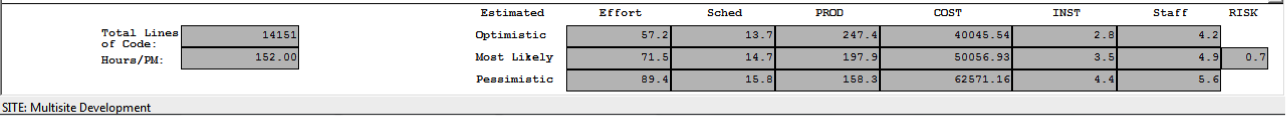
\includegraphics{COCOMOTODO1}} 
%\vspace{0.35cm}

\setcounter{section}{0}
\part{Introdución}
	\section{Propósito}
	Este documento pretende recopilar de manera clara y concisa todos los diagramas UML del Software KIKE HOSTELERIA ®, generados con la herramienta \texttt{Bouml}. Se pueden dividir en tres partes, cada una de ellas más cercana al código del lenguage de programación, y con mayor grado de detalle. Éstas son: Requisitos, análisis y diseño, partes fundamentales de este documento.

	\section{Audiencia} 
	La aplicación está pensada para hoteles y/o restaurantes de capacidad media/baja, pero podría ampliarse para capacidades mayores sin dificultad.

	El documento está pensado para dos audiencias distintas. En las primeras partes, sirve como lazo de comunicación entre el equipo (nosotros) y la empresa hostelera. Según se entra más en materia, centrándose en el Software, está pensado para el equipo de diseñadores y programadores.

	\section{Alcance}
	Todos los diagramas que se han requerido para la posterior codificación de la aplicación. Se añade, además, una breve explicación de los mismos, poniéndolos en contexto e indicando su naturaleza y significado.

	Todo el documento debe entenderse dentro del ámbito del UML y del modelo del Proceso Unificado, seguido durante todo el proyecto.

\section{Definiciones, acrónimos y abreviaturas}

	Todo lo referente a esta sección se encuentra en el documento anexo \texttt{Definiciones, acrónimos y abreviaturas}. Ahí se detallan las palabras poco comunes, los anglicísmos y abreviaturas que se emplean.

	\section{Referencias}
	Se han utilizado los diguientes recursos:
	\begin{itemize}
		\item Nuestro propio documento de \texttt{Documento de casos de uso}, así como \\ \texttt{Definiciones, acrónimos y abreviaturas}
		\item Apuntes de Clase de la asignatura “Ingeniería del Software" de la Universidad Complutense de Madrid, Curso 2012-2013
		\item \textbf{Booch, G.; Rumbaugh, J.; Jacobson, I. }. El lenguaje unificado de modelado (2006, 2ª edición).
		\item \textbf{Larman, C.}. UML y patrones (2003, 2ª edición).
		\item \textbf{Ambler, S. W.} The Elements of UML Style (2003).
	\end{itemize}

\newpage
\mbox{}
\thispagestyle{empty}						% Hoja en blanco, sin numeros ni nada
\newpage





\setcounter{section}{0}
\part{Requisitos}
	\section{Modelo de Dominio}
	En esta sección se recoge el modelo de dominio de toda la aplicación. De izquierda a derecha, podemos ver la relación entre el cliente y las reservas que puede hacer, tanto del restaurante como del hotel. A partir de ellas se puede genarar una factura. 

	Las reservas del hotel son atendidas por el recepcionista, y las del restaurante por el camarero (o en su defecto, el maître). El camarero, además tiene varias posibilidades, puede acceder y modificar la distribución de las mesas del restaurante, tomar o modificar comandas, ver o modificar el menú y ver o modificar las existencias de la cocina y el bar.

	En cuanto a la limpieza, el encargado asigna tareas de limpieza al personal de limpieza. Posteriormente, cuando se suponen completadas, el encargado revisa si se han cumplido los objetivos en dichos encargos, dando su visto bueno.

	Además, el encargado de mantenimiento puede ver las tareas que tiene pendientes por resolver en el hotel o el restaurante. Estas son notificadas por el resto de empleados (o el mismo, al ser un empleado más) cuando las descubren. Otro medio de comunicación entre los empleados son las notas. Cualquiera puede escribir una y cualquiera puede verlas. Su fin es distinto al de las obligaciones de mantenimiento, ya que pueden tratarse temas más triviales o que no tocan dichas tareas.
		
	Por último, el jefe del negocio tiene acceso a las cuentas de las cajas de la recepción y del restaurante, que se recogen en el libro diario de la aplicación. Éste, a su vez, se resume en el libro mayor.
	

	\section{Diagramas de actividad}






\setcounter{section}{0}
\part{Análisis}
	\section{Diagamas de paquetes}


	\section{Diagramas de comunicación}


	\section{Diagramas de clases de análisis}






\setcounter{section}{0}
\part{Diseño}
	\section{Diagramas de secuencia}


	\section{Diagramas de clases de diseño}


	\section{Diagramas de componentes}


	\section{Diagramas de despliegue}






\setcounter{section}{0}
\part{Patrones de diseño}



\newpage
\mbox{}
\thispagestyle{empty}						% Hoja en blanco, sin numeros ni nada al final del documento
\newpage

\end{document}